\chapter{\ifenglish Conclusions and Discussions\else บทสรุปและข้อเสนอแนะ\fi}

\section{\ifenglish Conclusions\else สรุปผล\fi}

Wazuh has successfully modernized the HAIT+ cybersecurity framework by transitioning it from a manual checklist into an automated, real‑time SIEM alerting pipeline. Leveraging Wazuh demonstrates that open‑source architectures can provide a highly customizable and cost‑effective solution that aligns with the budget constraints of district‑level hospitals. Ultimately, the \textit{Command‑to‑Rule} pipeline enables hospital IT staff to independently adapt and scale their monitoring capabilities in response to the evolving demands of new medical software and system performance metrics.

\section{\ifenglish Challenges\else ปัญหาที่พบและแนวทางการแก้ไข\fi}

One of the core challenges encountered in this project was that out‑of‑the‑box SIEM platforms do not inherently capture hospital‑specific operational requirements. To address this limitation, the \textit{Command‑to‑Rule} pipeline was developed. In this approach, Wazuh agents are configured to execute localized scripts, ingest the resulting output as generic logs, and apply custom regular‑expression (RegEx) rules on the manager to assign anomaly scores.

This design is highly scalable. When a hospital requires monitoring of a new process or metric, the administrator only needs to modify a single shell command on the agent, without altering or rebuilding the core alerting architecture.

\begin{itemize}
  \item \textbf{Challenge 1:} Misclassified Database Alerts \\
  Critical database events were incorrectly parsed and ingested as Apache Web Server logs, resulting in the suppression of important database-related alerts.

  \textbf{Solution:} A hierarchical rule structure (parent–child rules) was implemented to intercept the misclassified logs and reclassify them as Level 9 critical alerts based on specific database-related keywords.
  \begin{figure}[h!]
    \centering
    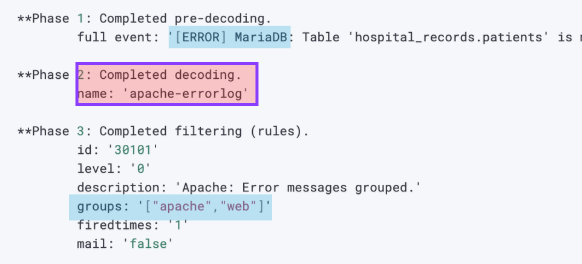
\includegraphics[width=\textwidth]{images/Challeng_10.png}
  \end{figure}

  \item \textbf{Challenge 2:} Unreliable Windows Event IDs \\
  Microsoft frequently modifies Event IDs during system updates, which reduces the reliability of native firewall monitoring mechanisms across different Windows versions.

  \textbf{Solution:} The monitoring strategy was shifted to command-line auditing (Event ID 4688). By monitoring the actual commands executed (for example, \texttt{netsh advfirewall}), the alerting logic remains consistent and effective across all supported Windows versions.
  \begin{figure}[h!]
    \centering
    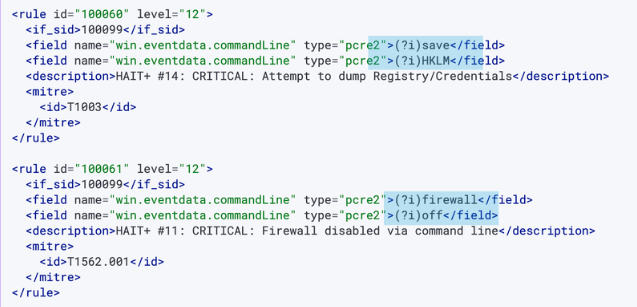
\includegraphics[width=\textwidth]{images/Challenge_20.png}
  \end{figure}
\end{itemize}

\section{\ifenglish%
Suggestions and further improvements
\else%
ข้อเสนอแนะและแนวทางการพัฒนาต่อ
\fi
}

While the current SIEM implementation successfully established a centralized monitoring baseline, several enhancements could further mature the system's capabilities. To achieve a more comprehensive defense-in-depth architecture and better align with broader cybersecurity compliance standards, the following future improvements by utilizing external tools are recommended.

\begin{itemize}
\item \textbf{Network Intrusion Detection (NIDS) Integration}\\
Future iterations of the project should integrate dedicated NIDS, such as Suricata or Zeek, alongside the existing Wazuh deployment. This integration would provide necessary telemetry to actively identify and resolve network congestion issues and unauthorized external device connections.

\item \textbf{Context-Aware Access Control via Cross-Departmental APIs}\\
A critical aspect of modern access control compliance is context. The SIEM's effectiveness can be significantly improved by shifting from static log analysis to dynamic, context-aware monitoring via API integrations with external organizational databases, thereby enabling user access monitoring.

\item \textbf{Physical and IoT Security Correlation}\\
Comprehensive security monitoring must bridge the gap between logical and physical infrastructure. Future development should expand the SIEM's ingestion capabilities to include telemetry from IoT devices and data center hardware such as SNMP and PDUs, allowing detection of abnormal power resource usage.
\end{itemize}
